\documentclass[11pt]{beamer}
\usetheme{Copenhagen}
\usepackage[utf8]{inputenc}
\usepackage[english]{babel}
\usepackage{amsmath}
\usepackage{amsfonts}
\usepackage{amssymb}
\usepackage{graphicx}
\usepackage{enumerate}
\usepackage{multimedia}
\usepackage{mathtools}
\DeclareMathOperator*{\argmin}{\mathrm{arg\, min}}
\usepackage{caption}
\usepackage{subcaption}
\author{Onofre Martorell, Lidia Talavera}
\title{Image inpainting and completion}
%\setbeamercovered{transparent} 
%\setbeamertemplate{navigation symbols}{} 
%\logo{} 
%\institute{} 
%\date{} 
%\subject{} 
\begin{document}

\begin{frame}
\titlepage
\end{frame}

%\begin{frame}
%\tableofcontents
%\end{frame}

\begin{frame}{Introduction}
\begin{block}{Goal of the project}
Restore the given image using variational and graphical models.
\end{block}

\begin{figure}
\begin{center}
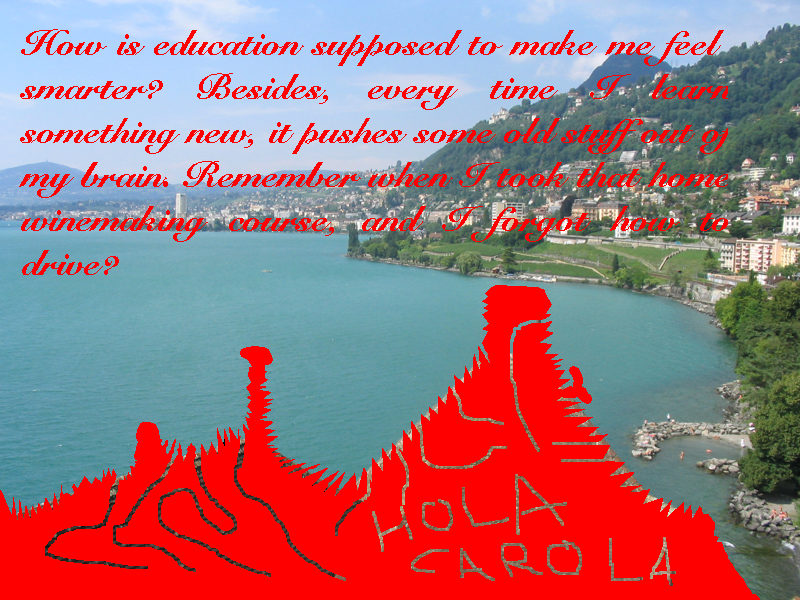
\includegraphics[scale=0.6]{Goal_image}
\end{center}
\end{figure}
\end{frame}

\begin{frame}{Introduction}
\begin{block}{Steps}
\begin{enumerate}
\item Image inpainting
\item Image segmentation
\item Poisson editing
\item Image completion
\end{enumerate}
\end{block}
\end{frame}


\begin{frame}
\frametitle{Image inpainting}

\begin{block}{Image inpainting}
Replace lost or corrupted data on images or videos.
\end{block}

\begin{exampleblock}{Example}
\begin{figure}
\begin{center}
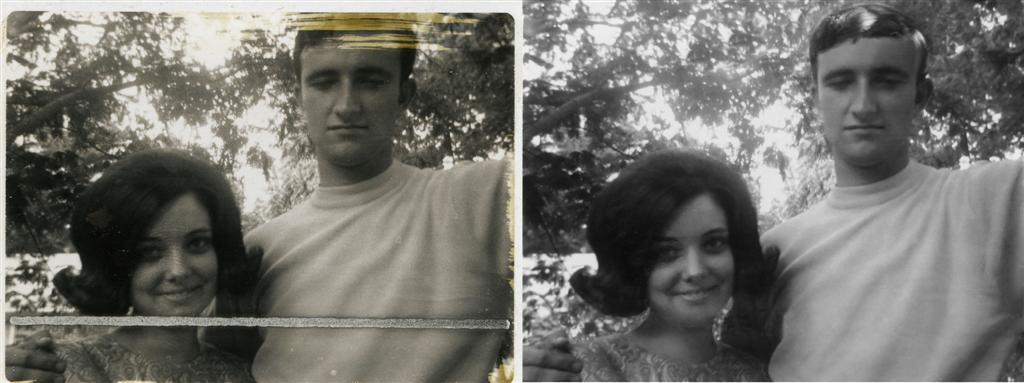
\includegraphics[scale=4.2]{Restoration}
\end{center}
\end{figure}
\end{exampleblock}
\end{frame}

\begin{frame}
\frametitle{Image inpainting}
\framesubtitle{Solution and implementation}
The problem of inpainting can be modelled as
$$
\begin{cases}
\displaystyle\argmin\limits_{u\in W^{1,2}(\Omega)}\int _D |\nabla u(x)|^2dx,\\
u|_{\partial D} = f
\end{cases}
$$
where $f$ is the image to inpaint.\\

The associated Euler-Lagrange equation of this functional is
$$\left\lbrace
\begin{array}{l l}

\Delta u = 0& \text{in }D \\
u = f & \text{in }\partial D

\end{array}\right.
$$
The equation is completed with homogeneous Neumann boundary
conditions at the boundary of the image.

\end{frame}
\begin{frame}
\frametitle{Image inpainting}
\framesubtitle{Solution and implementation}
\begin{block}{Discretization of Laplacian}
The Laplacian is discreticised using finite differences:
%\newline
\vfill
$$\frac{1}{h_j^2}u_{i,j-1} + \frac{1}{h_i^2}u_{i-1, j} - \bigg(\frac{2}{h_i^2}+\frac{2}{h_j^2}\bigg)u_{i,j} + \frac{1}{h_i^2}u_{i+1,j} + \frac{1}{h_j^2}u_{i, j+1} = 0$$
\vfill

%\newline
This is the equation that have to satisfy the pixels that we want to inpaint.
\end{block}
\end{frame}

\begin{frame}
\frametitle{Image inpainting}
\framesubtitle{Solution and implementation}
\begin{block}{Boundary conditions}
We have added one row or column to each side of the image and we have computed the Neumann boundary conditions. For example, at the east side, we get
$$\frac{u_{i, 1} - u_{i, 2}}{h_j} = 0\Longrightarrow u_{i,1} = u_{i, 2}$$

And for the pixels belonging to west, north or south boundary we have
$$ u_{i,n_j} = u_{i, n_j-1},\ u_{1,j} = u_{2, j}\ \text{or } u_{n_i,j} = u_{n_i-1, j}.$$
\end{block}

\begin{block}{Other pixels}
$$u_{i, j} = f_{i, j}$$
\end{block}
\end{frame}


\begin{frame}
\frametitle{Image inpainting}
\framesubtitle{Solution and implementation}
Ordering the pixels of the image as
$$x = (u_{1,1}, u_{2,1}, \cdots, u_{i, j}, u_{i+1, j}, \cdots ,u_{n_i + 2,n_j + 2})^T$$
the previous equations can be written as a linear system of equations 
$$Ax = b,$$
which can be solved using Matlab.
\end{frame}

\begin{frame}
\frametitle{Image inpainting}
\framesubtitle{Results}
\begin{figure}
    \centering
    \begin{subfigure}[b]{0.47\textwidth}
        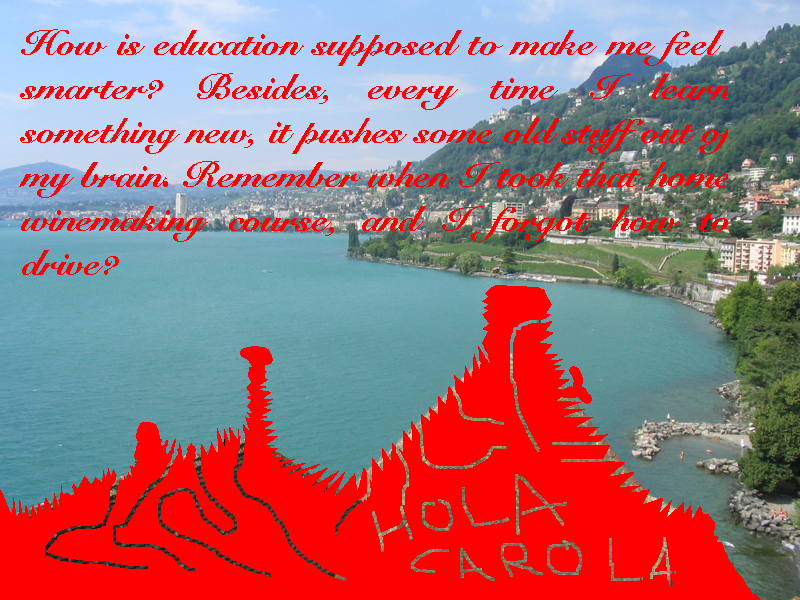
\includegraphics[width=\textwidth]{Image_to_Restore}

    \end{subfigure}
    ~ 
        \begin{subfigure}[b]{0.47\textwidth}
        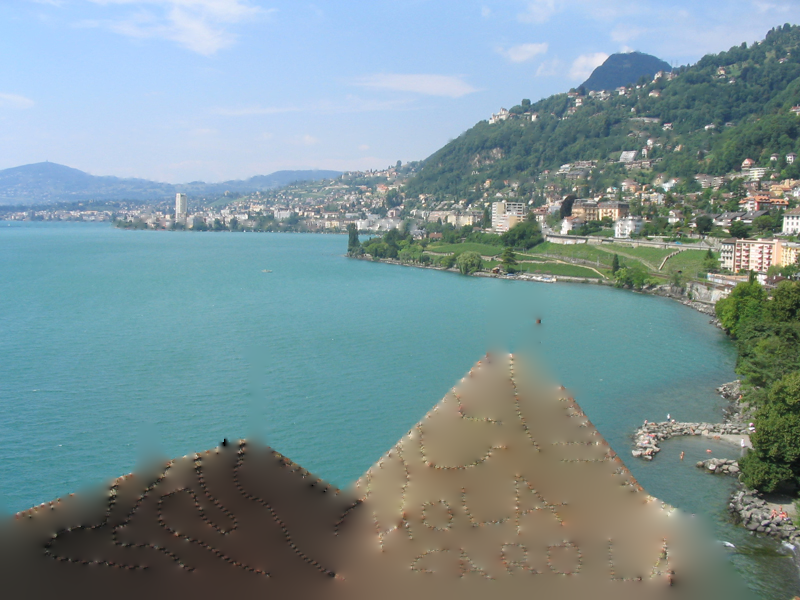
\includegraphics[width=\textwidth]{Goal_inpaint_bad}

    \end{subfigure}

\end{figure}
\end{frame}

\begin{frame}
\frametitle{Image inpainting}
\framesubtitle{Results}
\begin{figure}
    \centering
    \begin{subfigure}[b]{0.47\textwidth}
        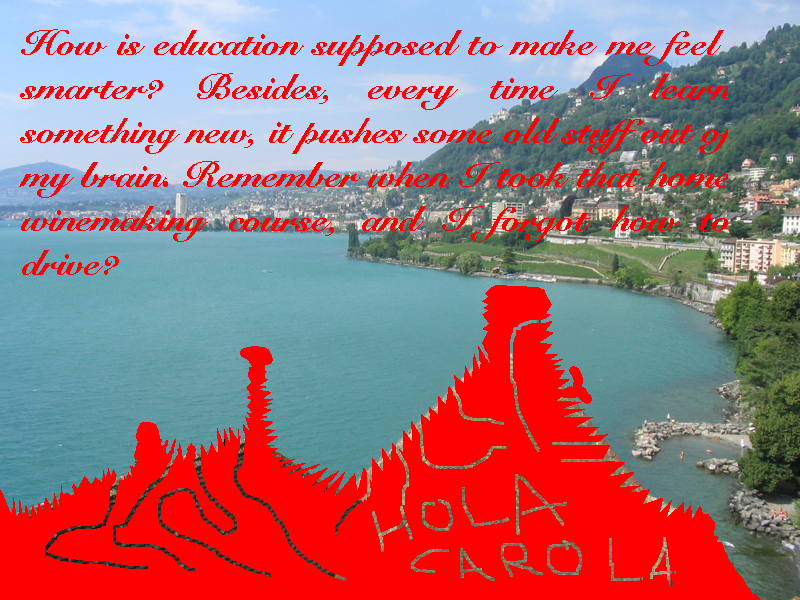
\includegraphics[width=\textwidth]{Image_to_Restore}

    \end{subfigure}
    ~ 
        \begin{subfigure}[b]{0.47\textwidth}
        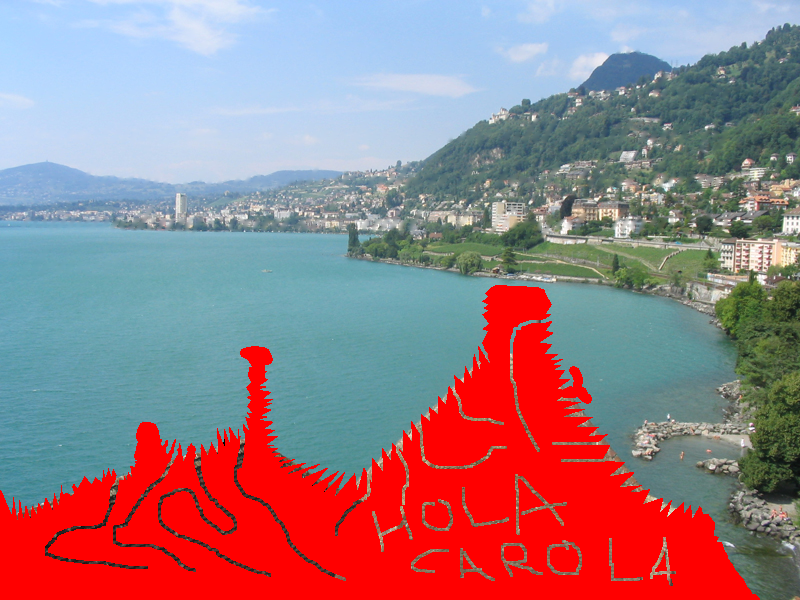
\includegraphics[width=\textwidth]{Goal_inpaint}

    \end{subfigure}

\end{figure}
\end{frame}

\begin{frame}
\frametitle{Image segmentation}

\begin{block}{Image segmentationn}
Divide the image into different parts.
\end{block}

\begin{exampleblock}{Example}
\begin{figure}
    \centering
    \begin{subfigure}[b]{0.36\textwidth}
        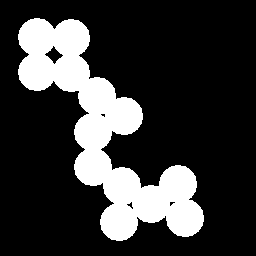
\includegraphics[width=\textwidth]{circles}

    \end{subfigure}
    ~ 
        \begin{subfigure}[b]{0.4\textwidth}
        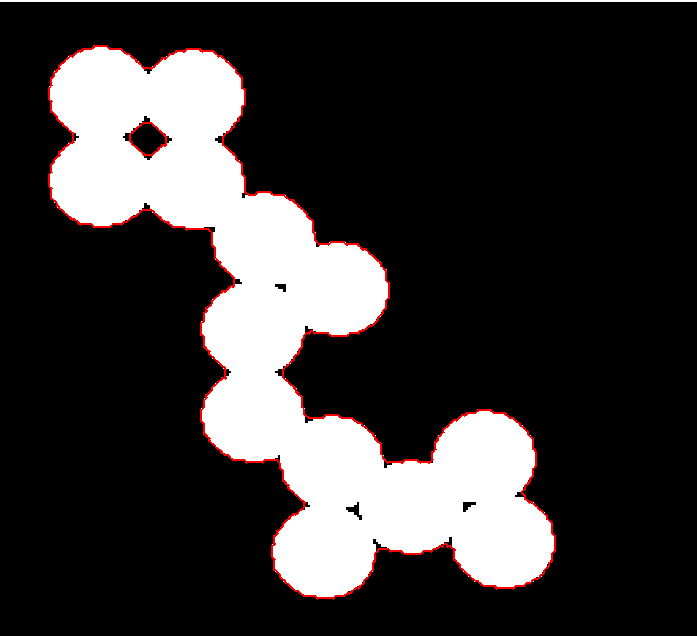
\includegraphics[width=\textwidth]{circles_segmented}

    \end{subfigure}

\end{figure}
\end{exampleblock}
\end{frame}

\begin{frame}
\frametitle{Image segmentation}
\framesubtitle{Solution and implementation}

We will use Chan-Vese segmentation which consist on finding a curve that is the boundary of the segmentation. The way to find that curve is minimizing the following functional:
$$\displaystyle\argmin\limits_{c_1, c_2, C}\ \mu \text{Lenght}(C) +\nu\text{Area}(inside(C)) +$$$$ \lambda_1\int_{inside(C)}|f(x)-c_1|^2dx + \lambda_2\int_{outside(C)}|f(x)-c_2|^2dx,$$
where $C$ is the boundary of a closed set and $c_1$, $c_2$ are the values of $u$ respectively inside and outside of $C$. 

\end{frame}

\begin{frame}
\frametitle{Image segmentation}
\framesubtitle{Solution and implementation}
\begin{block}{}
As it is difficult to manipulate $C$, Chan-Vese segmentation uses a function $\varphi$, where the curve $C$ will be the zero crossing of it, that is 
$$C = \{x\in \Omega:\varphi(x) = 0\}.$$
\end{block}

With this the functional is rewritten as:
$$\displaystyle\argmin\limits_{c_1, c_2, \varphi}\ \mu \int_{\Omega}\delta(\varphi(x))|\nabla\varphi(x)|dx+\nu \int_{\Omega}H(\varphi(x))dx +$$$$ \lambda_1\int_{\Omega}|f(x)-c_1|^2H(\varphi(x))dx + \lambda_2\int_{\Omega}|f(x) -c_2|^2(1-H(\varphi(x)))dx,$$
\end{frame}

\begin{frame}
\frametitle{Image segmentation}
\framesubtitle{Solution and implementation}
In the previous formula $H$ denotes the Heaviside function and $\delta$ the Dirac mass, its distributional derivative:
$$ H = \left\lbrace\begin{array}{l l}
1&t\geq 0,\\
0 & t<0
\end{array}\right. ,\quad \delta(t) = \frac{d}{dt}H(t).$$

Note that we cannot derive $H(t)$. Because of that, in the implementation we take the Heaviside function as
$$H_{\epsilon}(t) = \frac{1}{2}\bigg(1 + \frac{2}{\pi}\arctan \bigg(\frac{t}{\epsilon}\bigg)\bigg).$$

\end{frame}



\begin{frame}
\frametitle{Image segmentation}
\framesubtitle{Solution and implementation}
Now we have to minimize the functional respect to $c_1$, $c_2$ and $\varphi$.

The way to do it is the following: at each iteration we do this steps:
\begin{enumerate}
\item[1.] Update $c_1$ and $c_2$ as the average gray scale value where $\varphi$ is positive or negative, respectively.

\item [2.] Evolve $\varphi$ using the semi-implicit gradient descent 


\end{enumerate}
\begin{flushleft}
$
\begin{dcases}
\frac{\partial \varphi}{\partial t} = \delta_{\epsilon}(\varphi)\bigg[\mu \text{ div}\bigg(\frac{\nabla\varphi}{|\nabla\varphi|}\bigg) - \nu-\lambda_1(f-c_1)^2+\lambda_2(f-c_2)^2\bigg]\ \text{in }\Omega \\
\frac{\delta_{\epsilon}(\varphi)}{|\nabla\varphi|}\frac{\partial \varphi}{\partial \vec{n}} = 0\ \text{on }\partial\Omega 
\end{dcases}$
\end{flushleft}

\end{frame}
%$$\varphi_{i,j}^n = [\varphi_{i,j}^n + dt\cdot\delta_{\varepsilon}(\varphi_{i,j}^n)(A_{i,j}\varphi_{i+1,j}^n) + A_{i-1,j}\varphi_{i-1,j}^{n+1}+B_{i,j}\varphi_{i,j+1}^n+$$
%$$B_{i, j-1}\varphi_{i,j-1}^{n+1}-\nu - \lambda_1(f_{i,j}-c_1)^2+\lambda_2(_{i,j}-c_2)^2) ]/[1 + dt\cdot\delta_{\varepsilon}(\varphi_{i,j}^n)(A_{i,j} +$$$$ A_{i-1,j} + B_{i,j} + B_{i,j-1})]$$. 
\begin{frame}
\frametitle{Image segmentation}
\framesubtitle{Solution and implementation}
\begin{itemize}
\item [3.] Every certain number of iterations, reinitialize $\varphi$.
\item [4.] If we have reached the maximum number of iterations or the difference $\max(|\varphi^{n+1}-\varphi|)$ is lower than a given tolerance, we stop the algorithm.
\end{itemize}
\end{frame}


\begin{frame}
\frametitle{Image segmentation}
\framesubtitle{Results}
\begin{figure}
\begin{center}
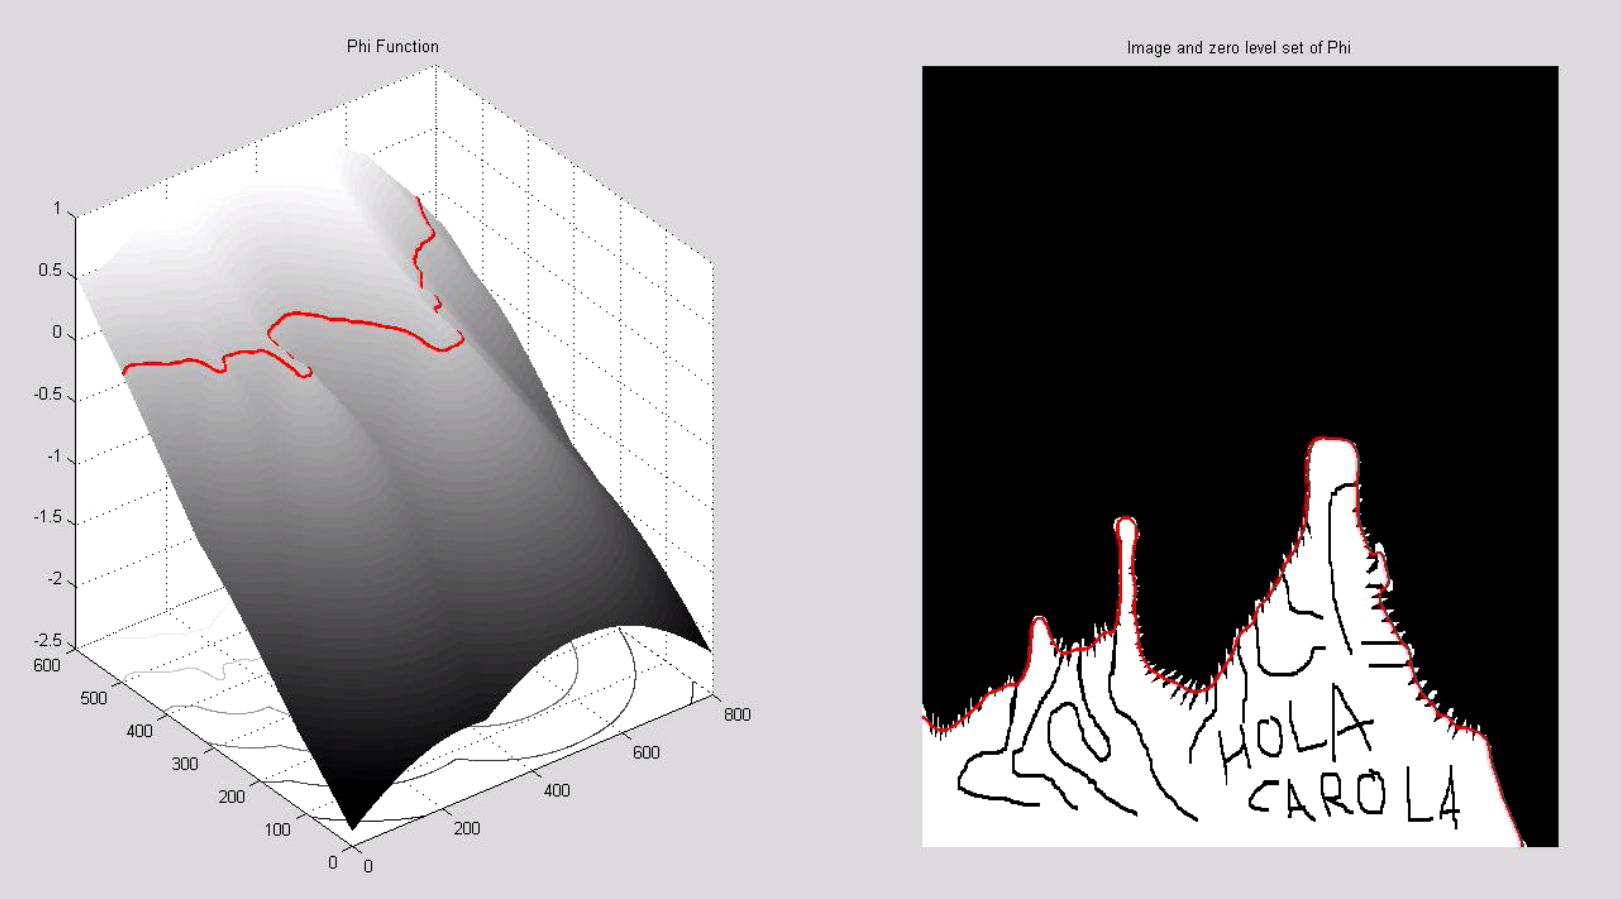
\includegraphics[scale=0.33]{Segmentation}


\end{center}
\end{figure}




\end{frame}


\begin{frame}
\frametitle{Poisson Image editing}

\begin{block}{Poisson Image editing}
Copy a region of an image to another one and adapt it in order that it does not seem fake.
\end{block}

\begin{exampleblock}{Example}
\begin{figure}
    \centering
    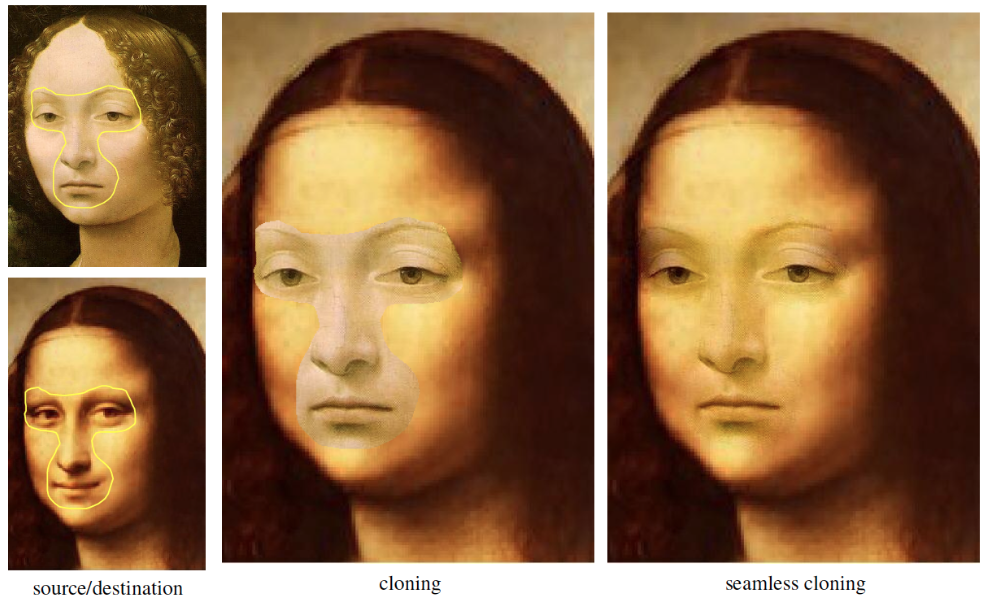
\includegraphics[width=70mm]{Example.png}
\end{figure}
\end{exampleblock}
\end{frame}

\begin{frame}
\frametitle{Poisson Image editing}
\framesubtitle{Solution and implementation}
Seamless cloning will be applied through the implementation of the importing gradients method. Let $f^{*}$ be the destination image, $f$ the source image that contains the region we want to clone, $\Omega$ which will be cloned from $f$ to $f^{*}$  and $\overrightarrow{v}$ the guidance field of vectors.\newline
\begin{figure}
\begin{center}
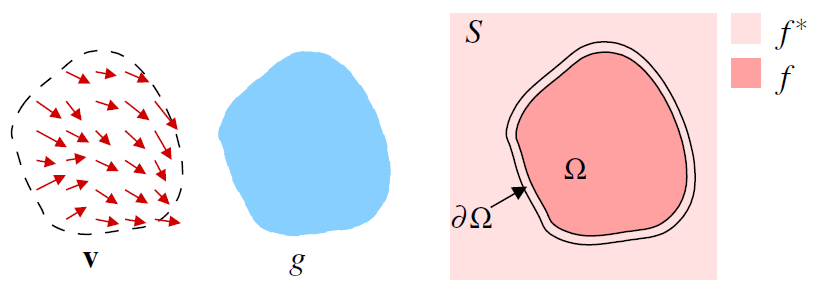
\includegraphics[scale=0.55]{Seamless_cloning}
\end{center}
\end{figure}
\end{frame}


\begin{frame}
\frametitle{Poisson Image editing}
\framesubtitle{Solution and implementation}
To solve the problem we have used the next functional over each channel of the image:
\begin{equation*}
\min_{f}\int_{\Omega }\left | \nabla f-\overrightarrow{v} \right |^{2},
\label{eq:functional}
\end{equation*}

with $f_{\mid \delta \Omega}=f_{\mid \delta \Omega}^{*}$, \newline

The associated Euler-Lagrange of this functional is

\begin{equation*}
\left\{\begin{matrix}
 \Delta f=div \overrightarrow{v} & \text{on } & \Omega\\ 
 f=f^{*}& \text{in }\partial\Omega
\end{matrix}\right.
\label{eq:Poisson_general}
\end{equation*}
\end{frame}

\begin{frame}
\frametitle{Poisson Image editing}
\framesubtitle{Solution and implementation}
We are using importing gradients, which means that the guidance field $\overrightarrow{v}$ is a gradient field taken directly from a source image. Denoting
by $g$ the source image, this is
$$\overrightarrow{v} = \nabla g.$$

Replacing this, we get
\begin{equation*}
\left\{\begin{matrix}
 \Delta f=\Delta g & \text{on } & \Omega\\ 
 f=f^{*}& \text{in }\partial\Omega
\end{matrix}\right.
\end{equation*}
%_{\mid \partial \Omega}
%_{\mid \partial \Omega}

What we have done is the following: we have taken the code of the previous week and we have changed it in order to detect if there is a variable containing the discretization of $\Delta g$ for each point of the image. If this variable exists, it computes $\Delta f = \Delta g$; otherwise it computes $\Delta f = 0$.
\end{frame}

\begin{frame}
\frametitle{Poisson Image editing}
\framesubtitle{Results}
\begin{figure}
    \centering
    \begin{subfigure}[b]{0.36\textwidth}
        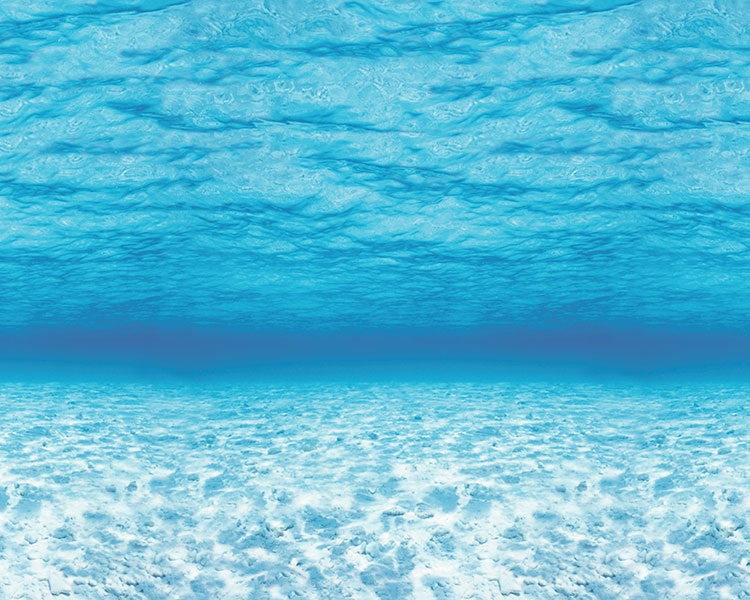
\includegraphics[width=\textwidth]{the_sea}

    \end{subfigure}
    ~ 
        \begin{subfigure}[b]{0.4\textwidth}
        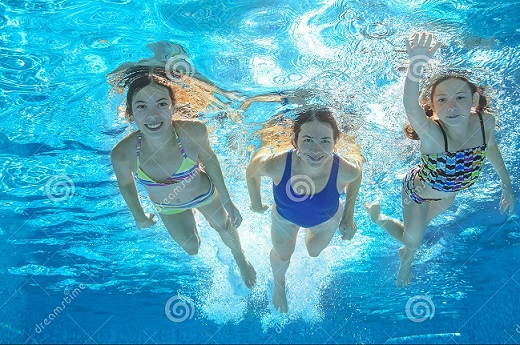
\includegraphics[width=\textwidth]{family}

    \end{subfigure}



\end{figure}

\begin{figure}
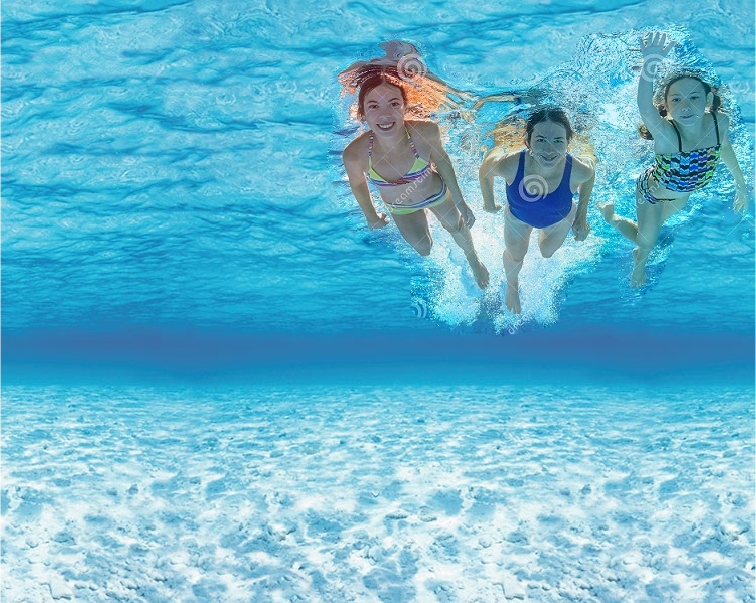
\includegraphics[width=0.4\textwidth]{family_sea}
\end{figure}
\end{frame}




\begin{frame}
\frametitle{Image completion}

\begin{block}{Image completion}
Select a similar image to the given one and copy a selected region.
\end{block}

%\begin{exampleblock}{Example}
%\end{exampleblock}
\end{frame}

\begin{frame}
\frametitle{Image completion}
\framesubtitle{Solution and implementation}
\begin{itemize}
\item [1.]  From a huge database of image, find the most similar images using GIST descriptors.
\item [2.] From every found image, find the most similar region to the hole of our image.
\item [3.] Authomatically fine tune of the editing mask. This step consists on taking the segmentation obtained  and tuning it using a graphical model.
\end{itemize}
\end{frame}

\begin{frame}
\frametitle{Image completion}
\framesubtitle{Solution and implementation}
The cost function used is
\begin{equation*}
C(L) = \sum_pC_d(p, L(p)) + \sum_{p, q}C_i(p, q, L(p), L(q))
\end{equation*}
where 
\begin{itemize}
\item $L(p)$ is the label of the pixel $p$: \emph{exists} or \emph{patch}.
\item $C_d$ are the unary potentials:
\begin{itemize}
\item If $p$ belongs to the mask, $C_d(p, \text{\emph{exists}}) = \infty$ and $C_d(p, \text{\emph{patch}}) = 0$
\item If $p$ does not belong to the mask, $C_d(p, \text{\emph{exists}}) = 0$ and $C_d(p, \text{\emph{patch}}) = (k\cdot(\text{dist}(p, \text{mask}))^3$
\end{itemize}


\item $C_i$ are the binary potentials: if the pixels are adjacent and have different label, its value is the difference of the SSD at each pixel.
\end{itemize}
\end{frame}

\begin{frame}
\frametitle{Image completion}
\framesubtitle{Solution and implementation}
\begin{itemize}
\item [4.] Copy the region to our image and perform Poisson Editing correction.
\item [5.] As we will have many results, choose by visual inspection the best one.
\end{itemize}
\end{frame}

\begin{frame}
\frametitle{Image completion}
\framesubtitle{Results}

\end{frame}


\begin{frame}{Conclusions}
\begin{itemize}
\item We have solved our problem in different techniques that at the beginning didn't seem to be related among them.
\item During the project, we have learned how to solve some variational and graphical models.

\end{itemize}
\end{frame}

\begin{frame}
\begin{block}{}
\centering
\Large Any questions?
\end{block}
\end{frame}
\end{document}